\begin{figure*}[t] %[!b]
    \centering
    \vspace{-10pt}
    %\scalebox{.9}{
    \begin{subfigure}[t]{0.31\linewidth}
        \centering
        \fbox{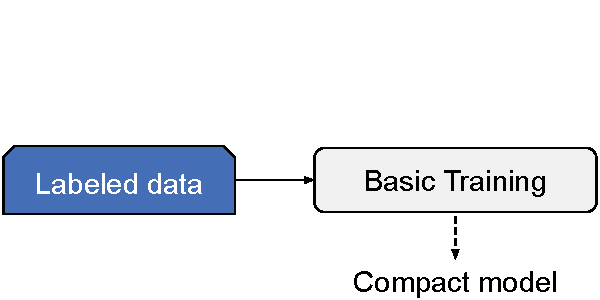
\includegraphics[width=\columnwidth]{figures/recolored_vanilla_training.pdf}}
        \caption{Basic Training}
        \label{fig:baseline-vanilla-training}
    \end{subfigure}
    \hspace{0.3cm}
    \begin{subfigure}[t]{0.31\linewidth}
        \centering
        \fbox{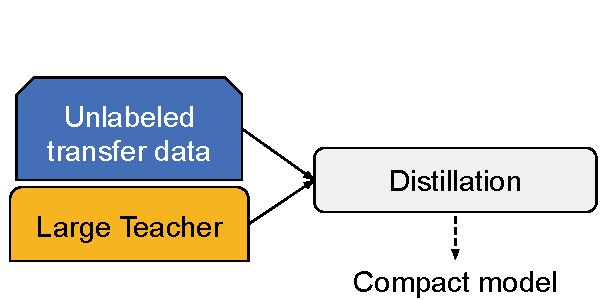
\includegraphics[width=\columnwidth]{figures/recolored_knowledge_distillation.pdf}}
        \caption{Distillation}
        \label{fig:baseline-distillation}
    \end{subfigure}
    \hspace{0.3cm}
    \begin{subfigure}[t]{0.31\linewidth}
        \centering
        \fbox{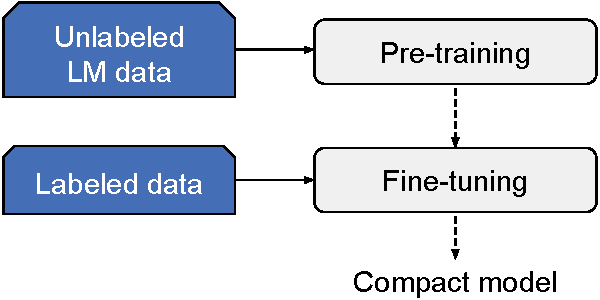
\includegraphics[width=\columnwidth]{figures/recolored_pre-training.pdf}}
        \caption{\PtFt (PF)}
        \label{fig:baseline-pretraining}
    \end{subfigure}
    %}
    \caption{Baselines for building compact models, used for analysis (Section \ref{sec:exp}).}
    \label{fig:training-strategies}
    \vspace{-10pt}
\end{figure*}